\section{Background}

The original intent behind the web was to share documents written in HTML, CSS that used JavaScript for simple tasks such as client-side form validation \parencite{Moller2018,Zakai2018}.

% JavaScript is today well supported in virtually all web browsers on both desktop and mobile \parencite{Zakai2011}.

% The last few years more advanced applications has moved to the web, mandating higher performance (REF).

\subsection{Web apps}

Historically programs or applications run locally on a client device such as a personal computer. Since the introduction of the iPhone in 2007 and the release of the iOS app store in 2008 followed by the introduction of Google Play later the same year many %use numbers here?
has gotten acquainted with mobile apps, applications that run locally on a mobile device.

Wep applications, or web apps for short, is a type of application that run inside a web browser. Traditionally web applications a built with a thin user interface layer through which the user interacted with the application, while the actual computation was executed on one or more servers, % in the cloud
passing data back and forth between the client and the server.

Web apps are based on HTML, CSS, and JavaScript \parencite{ParkJungMoon2015}, the same web technologies originally conceived to share documents. JavaScript is increasingly popular for building high performance web apps \parencite{SandhuHerreraHendren2018}

web apps have an advantage of portability compared to mobile apps, but given the foundation of JavaScript is lacking in performance.

. Web applications are made possible through use of JavaScript, but according to \textcite{ParkJungMoon2015} the dynamic typing and prototypes features of JavaScript makes it execution inefficient. 

''JavaScript is the most widely used language for web programming, and now increasingly becoming popular for high performance computing, data-intensive applications, and deep learning. More recently, WebAssembly has been introduced as a typed low-level by'' \parencite{SandhuHerreraHendren2018}


According to \textcite{ParkJungMoon2015} 



\textcite{HaasRossbergSchuffTitzerHolmanGohmanWagnerZakaiBastien2017} notes that while the web has given rise to demanding web apps JavaScript as a language, being the only programming language available in web browsers, is not very well equipped to support such applications.

However according to \textcite{ReiserBlaser2017} there is always a desire for higher performance. \textcite{Zakai2018} describes JavaScript as an obstacle for demanding/truly high-performing applications/apps.

\subsection{JavaScript}

JavaScript was introduced 1995 with the intention to solve small tasks, e.g. validation of input data and small animations. The last few years the web has evolved from simply being a platform for websites to also be a platform for (webb-)applications/apps.

JavaScript was a major addition to the set of web technologies. It is estimated that X \hl{add numbers with references here} use JavaScript.

[...]



''One popular way of accelerating JavaScript is using the just-in-time compilation (JITC), which translates the JavaScript source code to the machine code at runtime. Unfortunately, JavaScript JITC for web apps suffers from the parsing and compilation overhead seriously, which offsets the performance gain of executing the compiled code.'' \parencite{ParkJungMoon2015}


\begin{figure}[!h]
\centering
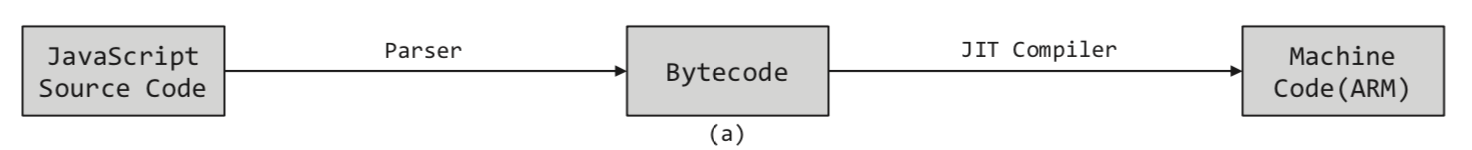
\includegraphics[width=16cm,keepaspectratio]{jit-compiling-ParkJungMoon2015}
\caption{JavaScript interpretation. (to be) Adapted from \textcite{ParkJungMoon2015}}
\label{figure:label}
\end{figure}    

\begin{lstlisting}[label=lst1,language=JavaScript,numbers=none,caption=prototype.js,frame=none]
Name.prototype = {
    methodName: function(params){
        var doubleQuoteString = "some text";
        var singleQuoteString = 'some more text';
        // this is a comment
        if(this.confirmed != null && typeof(this.confirmed) == Boolean && this.confirmed == true){
        document.createElement('h3');
        $('#system').append("This looks great");
        return false;
        } else {
        throw new Error;
        }
    }
}
\end{lstlisting}

Listing \ref{lst1}

\subsubsection*{Optimizing/ations}

[...]

A major problem with optimizing is that fact that JavaScript is a loosely typed language, which means that the interpreter needs to be able to store any type of data in any variable. If the interpreter instead would be able to distinguish between which type of data each variable can store, it would be much easier to optimize.

\subsubsection*{JIT}

''One popular way of accelerating JavaScript is using the just-in-time compilation (JITC), which translates the JavaScript source code to the machine code at runtime. Unfortunately, JavaScript JITC for web apps suffers from the parsing and compilation overhead seriously, which offsets the performance gain of executing the compiled code.'' \parencite{ParkJungMoon2015}

The manufacturers of web browsers has in the last few years focused on optimizing JavaScript performance in different ways, such as introducing ''Just-In-Time'' (JIT) compilers \parencite{HerreraChenLavoieHendren2018}.

\subsubsection*{AOT}



\subsubsection*{TypeScript}

TypeScript \hl{REF} is a superset of JavaScript that adds type information. Type information allows the programmer to see mistakes sooner during the development phase rather than later in runtime.

\begin{lstlisting}[label=listing:typescript,language=JavaScript,numbers=none,caption=prime.ts,frame=none]
function isPrime(value: number) {
    for(var i = 2; i < value; i++) {
        if(value % i === 0) {
            return false;
        }
    }
    return value > 1;
}
\end{lstlisting}

This does not directly solve the problem, but decreases the number of runtime errors, and enables future backend optimizations such as improved guesses by the JIT-compiler.

% if there should be any subsubsection section shown in the table of contents it should be asm.js
\subsubsection{asm.js}

asm.js is a subset of JavaScript that is known to be heavily optimized. The main part of the optimization is ...

''A key development here is asm.js,1 which in 2013 was introduced in the Firefox browser. The idea behind asm.js is that JavaScript is slow because it is very dynamic and com- plex, so if we define a subset of JavaScript that is simple, it could be far more easily optimized,'' \parencite{Zakai2018}

\begin{lstlisting}[label=listing:asmjs,language=JavaScript,caption=asm.js]
function strlen(ptr) { // calculate length of C string
    ptr = ptr|0;
    var curr = 0;
    curr = ptr;
    while (MEM8[curr]|0 != 0) {
        curr = (curr + 1)|0;
    }
    return (curr - ptr)|0;
}
\end{lstlisting}

\begin{figure}
    \begin{small}
    \begin{verbatim}
function strlen(ptr) {
    ptr = ptr|0;
    var curr = 0;
    curr = ptr;
    while (MEM8[curr]|0 != 0) {
        curr = (curr + 1)|0;
    }
    return (curr - ptr)|0;
}
    \end{verbatim}
    \end{small}
    \caption{My Caption}
    \label{my-label}
\end{figure}

Listing \ref{listing:asmjs} shows an implementation of a C string calculation length function written in asm.js.

There are transpilers between JavaScript and asm.js such as EmScripten.

\paragraph{x}

x

\subparagraph{y}

y

\subsection{WebAssembly}

''WebAssembly is a new low-level language currently being implemented in all major web browsers. It is designed to become the universal compilation target for the web, obsolet- ing existing solutions in this area, such as asm.js and Native Client.'' \parencite{Watt2018}

WebAssembly\footnote{https://webassembly.org/} (Wasm) is by definition according to \textcite{HaasRossbergSchuffTitzerHolmanGohmanWagnerZakaiBastien2017} a portable assembly-language for web browsers and future adaptations. Technically WebAssembly is bytecode created by \emph{compiling} (any form of) code to WebAssembly \parencite{Watt2018} which then can be executed in any WebAssembly-engine. This can be compared with JavaScript-code that is \emph{interpreted} while running inside a JavaScript-engine.

WebAssembly can be seen as a successor to earlier technologies such as asm.js from Mozilla and Native Client (NaCL) from Google. NaCL executes native code in a separate part of Chrome and asm.js  \parencite{Zakai2018} is a subset of JavaScript optimized for performance \parencite{VanEsNicolayStievenartDHondtDeRoover2016} and can be interpreted in any web browser.

Earlier work on what today is WebAssembly has also resulted in EmScripten \parencite{Zakai2011}, a compiler based on LLVM \parencite{LattnerAdve2014} that originates as a transpiler from JavaScript to asm.js \parencite{Zakai2011} that has been further developed \parencite{HaasRossbergSchuffTitzerHolmanGohmanWagnerZakaiBastien2017} and is now able to compile both JavaScript and C/C++ to both asm.js and WebAssembly. EmScripten is the most common compiler to compile WebAssembly.

WebAssembly is the result of joint research and development between Apple, Google, Microsoft and Mozilla \parencite{HaasRossbergSchuffTitzerHolmanGohmanWagnerZakaiBastien2017}. WebAssembly has as the first technology since JavaScript full support in Chrome, Edge, Firefox and Safari. Those web browsers that does not support WebAssembly can according to \textcite{HaasRossbergSchuffTitzerHolmanGohmanWagnerZakaiBastien2017} use asm.js as ''polyfill''. WebAssembly is already being used where performance is of high importance, such as to generate cryptocurrency \parencite{RuthZimmermannWolsingHohlfeld2018}.

Initially WebAssembly supports code written in C/C++ \parencite{HaasRossbergSchuffTitzerHolmanGohmanWagnerZakaiBastien2017}. 
The focus on C/C++ is largely based on WebAssembly implementation limitations such as the lack of garbage collection. According to \textcite{HaasRossbergSchuffTitzerHolmanGohmanWagnerZakaiBastien2017} its a highly prioritized goal to allow WebAssembly to gain to access the web browsers built in garbage collector and that way support languages that use garbage collection.

WebAssembly is loaded as a module via a JavaScript API or another WebAssembly module \parencite{HaasRossbergSchuffTitzerHolmanGohmanWagnerZakaiBastien2017}. It's \emph{not} a goal to have WebAssembly replace JavaScript\footnote{https://webassembly.org/docs/faq/\#is-webassembly-trying-to-replace-javascript}, the idea is that they \emph{complement} each other. One example of how JavaScript and WebAssembly could complement each other is to replace large portions of JavaScript within popular JavaScript-frameworks with WebAssembly, but keep the JavaScript API towards the developer and thus only provide the benefit of performance.

WebAssembly is new technology. The first articles about WebAssembly was published in 2017 \parencite{HaasRossbergSchuffTitzerHolmanGohmanWagnerZakaiBastien2017,ReiserBlaser2017}.

\subsection{Benchmarking}

\parencite{LehmannPradel2018,MalleGiulianiKiesebergHolzinger2018}

[...]

WebAssembly is according to \textcite{HaasRossbergSchuffTitzerHolmanGohmanWagnerZakaiBastien2017} an option to JavaScript with higher performance. Higher performance makes way for demanding/truly high-performing applications/apps.
